\documentclass[11pt]{article}

% Color package
\usepackage{xcolor}

% Color scheme definitions
\definecolor{minimal-main}{HTML}{131313}
\definecolor{minimal-light}{HTML}{F2F2F2}
\definecolor{minimal-contrast}{HTML}{F3F2F5}
\definecolor{minimal-black}{HTML}{131313}
\definecolor{minimal-white}{HTML}{F3F2F5}
\definecolor{minimal-red}{HTML}{C43C2D}
\definecolor{minimal-blue}{HTML}{343454}
\definecolor{minimal-yellow}{HTML}{F1C40F}

% Colorbox environments
\usepackage[most]{tcolorbox}

% Page layout (A4)
\usepackage[paperheight=842pt, paperwidth=595pt, margin=0pt]{geometry}

% Remove paragraph indentation
\setlength{\parindent}{0pt}

% Interline spacing options
\newcommand{\largespace}{\\[2pt]}
\newcommand{\mediumspace}{\\[-3pt]}
\newcommand{\smallspace}{\\[-5pt]}

% In-box spacing around content
\newcommand{\inboxspacing}{.015\paperheight}

% Horizontal spacing of the boxes (must sum up to 1)
\newcommand{\sideboxwidth}{.35}
\newcommand{\mainboxwidth}{.65}

% Vertical spacing of the boxes (must sum up to 1)
\newcommand{\headboxheight}{.080}
\newcommand{\sideboxheight}{.910}
\newcommand{\aboutboxheight}{.120}
\newcommand{\mainboxheight}{.800}
\newcommand{\footboxheight}{.010}

% Typesetting packages
\usepackage[letterspace=20]{microtype}
\usepackage[T1]{fontenc}

% Raleway font family
\usepackage[semibold]{raleway}
\renewcommand{\familydefault}{\sfdefault}

% Custom font commands
\newcommand{\header}[2]{\uppercase{\textbf{\fontsize{30}{100}{\lsstyle{#1 \hspace{3pt} #2}}}}}
\newcommand{\titlefont}[1]{\uppercase{\textbf{\Large{#1}}}}

% Multirow tables
\usepackage{multirow}

% Settings for entire table columns
\usepackage{array}

% Tikzpicture graphics
\usepackage{tikz}

% Clickable URLs
\usepackage{hyperref}
\urlstyle{same}

% Expand span of tables
\usepackage{tabularx}

\begin{document}

\begin{tcbposter}[
    poster = {columns=1, rows=1, spacing=0pt},
    boxes = {sharp corners, halign=center, valign=center, boxrule=0pt}
]


% -- Headbox

\posterbox[
    colback=minimal-main,
    halign=center]
    {name=headbox,
    span=1,
    rowspan=\headboxheight}
{

    \color{white}

    \header{Mario}{Gonzalez}

    \vspace{-7px}
    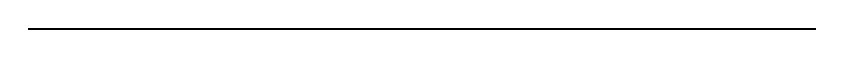
\begin{tikzpicture}
        \draw[fill=white] (-5.0, -0.01) rectangle (5.0, 0.01);
    \end{tikzpicture}
    \vspace{5px}

    \titlefont{Sofware \& Hardware Engineering}
}


% -- Sidebox
\posterbox[
    colback=minimal-light,
    valign=top,
    top=\inboxspacing,
    halign=left,
    right=\inboxspacing]
    {name=sidebox,
    below=headbox,
    column=1,
    span=\sideboxwidth,
    rowspan=\sideboxheight}
{
    \begin{tabular}{rl}
        \multicolumn{2}{@{}c@{}}{\includegraphics[scale=0.25]{images/pic.png}} \\
        \mediumspace

        & \titlefont{Contact} \\
        \hline \mediumspace

        \multirow{4}{*}{\scalebox{0.075}{\input{flags/switzerland.tex}}}
            & \textbf{Address} \\
                & ########### \\
                & ########### \\
                & ########### \\
                & \smallspace

        \multirow{2}{*}{\scalebox{0.075}{\input{icons/phone.tex}}}
            & \textbf{Phone} \\
                & \href{tel:+###########}{###########} \\
                & \smallspace

        \multirow{2}{*}{\scalebox{0.075}{\input{icons/email.tex}}}
            & \textbf{E-Mail} \\
                & \href{mailto:###########}{###########} \\
                & \largespace

        & \titlefont{Personal} \\
        \hline \mediumspace

        \multirow{2}{*}{\scalebox{0.075}{\input{icons/birthday.tex}}}
            & \textbf{Date of Birth} \\
                & ########### \\
                & \smallspace

        \multirow{2}{*}{\scalebox{0.075}{\input{icons/nationality.tex}}}
            & \textbf{Nationality} \\
                & ########### \\
                & \largespace

        & \titlefont{Platforms} \\
        \hline \mediumspace

        \multirow{2}{*}{\scalebox{0.075}{\input{icons/github.tex}}}
            & \textbf{GitHub} \\
                & \href{https://github.com/gonlezmario}{gonlezmario} \\
                & \smallspace

        \multirow{2}{*}{\scalebox{0.075}{\input{icons/linkedin.tex}}}
            & \textbf{LinkedIn} \\
                & \href{https://www.linkedin.com/in/gonlezmario/}{gonlezmario} \\
                & \largespace

        & \titlefont{Languages} \\
        \hline \mediumspace

        \multirow{2}{*}{\scalebox{0.075}{\input{flags/spain}}}
            & \textbf{Spanish} \\
                & Native \\
                & \smallspace

        \multirow{2}{*}{\scalebox{0.075}{\input{flags/britain.tex}}}
            & \textbf{English} \\
                & Proficient \\
                & \smallspace

        \multirow{2}{*}{\scalebox{0.075}{\input{flags/germany.tex}}}
            & \textbf{German} \\
                & Fluent \\
                & \smallspace

        \multirow{2}{*}{\scalebox{0.075}{\input{flags/france.tex}}}
            & \textbf{French} \\
                & Beginner

    \end{tabular}}

% -- Aboutbox
\posterbox[
    colback=white,
    valign=center,
    top=\inboxspacing,
    halign=left,
    right=\inboxspacing]
    {name=aboutbox,
    below=headbox,
    column*=1,
    span=\mainboxwidth,
    rowspan=\aboutboxheight}
{
    \textbf{Passionate electronics engineer with a keen interest in embedded systems, clean code practices, hardware design, and control engineering.}
}

% -- Mainbox
\posterbox[
    colback=white,
    valign=top,
    top=\inboxspacing,
    halign=left,
    left=\inboxspacing]
    {name=mainbox,
    column*=1,
    span=\mainboxwidth,
    below=aboutbox,
    rowspan=\mainboxheight}
{
    \begin{tabular}{>{\footnotesize}rl}
        & \titlefont{Work Expericence} \\
        \hline \mediumspace

        11/2022 - Currently
            & \textbf{Solexperts AG} \\
            & \textbf{Software Developer} \\
            & IoT platform development and maintenance \\
            & Data acquisition software development \\
            & Software migration and update \\
            & \smallspace

        04/1818 - 08/1826
            & \textbf{Nippon Gases} \\
            & \textbf{Engineering Intern} \\
            & Write and translate technical internal documentation\\
            & Requirements-Engineering \\
            & \largespace

        04/1818 - 08/1826
            & \textbf{CID Kids} \\
            & \textbf{It Teacher} \\
            & Introduced coding and electronics to children\\
            & and teenagers during a summer tech camp \\
            & Prepared lectures and electronic circuits \\
            & \largespace

        & \titlefont{Education} \\
        \hline \mediumspace

        2017 - 2022
            & \textbf{University of Oviedo} \\
            & \textbf{Industrial Electronic and Automatic Engineering} \\
            & Bilingual Itinerary (240 ECTS)\\
            & Energy Efficient Electronics Especialization\\
            & \smallspace

        2019 - 2020
            & \textbf{Liverpool John Moores University} \\
            & \textbf{Electrical and Electronic Engineering} \\
            & Erasmus+ Scholarship \\
            & First Honours \\
            & \largespace
    \end{tabular}
    
    \begin{tabularx}{\textwidth}{Xl}
    \titlefont{Soft Skills} & \titlefont{Hard Skills} \\
    \hline \mediumspace
    Communication & Python \\
    Problem-Solving & C/C++ \\
    Flexibility & IoT \\
    Attention to Detail & PCB Design \\
    Continuous Learning & Linux \\
    \smallspace
\end{tabularx}
}

% -- Footbox
\posterbox[colback=minimal-main]
           {name=footbox,
           below=sidebox,
           span=1,
           rowspan=\footboxheight}{}

\end{tcbposter}
\end{document}
